\chapter{\IfLanguageName{dutch}{Stand van zaken}{State of the art}}%
\label{ch:stand-van-zaken}

% Tip: Begin elk hoofdstuk met een paragraaf inleiding die beschrijft hoe
% dit hoofdstuk past binnen het geheel van de bachelorproef. Geef in het
% bijzonder aan wat de link is met het vorige en volgende hoofdstuk.

% Pas na deze inleidende paragraaf komt de eerste sectiehoofding.

\section{Inleiding}

Dit onderzoek start met een grondige onderdompeling in de wereld van telecommunicatie en technologie om zo een volledige literatuurstudie op te stellen. Verscheidene onderwerpen zullen aan bod komen zoals de geschiedenis van cellulaire netwerken, zodat er een duidelijk beeld kan gevormd worden van de verscheidene evoluties die netwerken hebben doorgaan om de kwaliteit van vandaag te leveren. Daarnaast zal ook een LTE netwerk specifiek besproken worden omdat dit het type is dat men zal inzetten gedurende de test opstelling. Hierna zal dan verdergegaan worden op allerlei termen die vaak voorkomen wanneer men de kwaliteit van een bepaald signaal bespreekt.

\section{Geschiedenis van het cellulair netwerk}

\subsection{Eerste generatie}

1G werd geïntroduceerd in de wereld in 1979. Deze technologie, eerst gebruikt door de inwoners van Japan, bracht de mogelijkheid om anderen te bellen maar het had ook een groot deel aan nadelen. Zo was een gesprek niet beveiligd, was roaming niet mogelijk en de geluidskwaliteit was zeer laag.
De reden dat een gesprek niet beveiligd is vanwege het feit dat er geen encryptie is over het netwerk dus eender wie die wou, kon meeluisteren. De trage downloadsnelheid die hier vernoemd werd bedroeg 2.4 kbps \autocite{Galazzo2020}. Neem nu bijvoorbeeld een korte film van 10 minuten in een mp4 formaat met codec H264 en een resolutie van 1920 x 1080p met een bitrate van 10.000 kbit/s. Zo'n bestand zou 775 MB in nemen. \autocite{Helme2019} De tijd dat het dus zou nemen om dit bestand te downloaden over het medium dat momenteel besproken word komt neer op 28 dagen, 22 uur, 26 minuten en 40 seconden. \autocite{Wooding2024}

\subsection{Tweede generatie}

2G maakte zijn introductie in de wereld gedurende het jaar 1991 in Finland op de rug van het Global System voor Mobile Communications of afgekort GSM. \autocite{Galazzo2020}. Deze volgende stap definieerde een significante stap naar verbetering ten opzichte van de eerste generatie. Men kon namelijk eindelijk berichten versturen naast bellen. Ook kon men multimedia bestanden delen zoals foto's en waren gesprekken vanaf dit punt wel geëncrypteerd en dus veilig van andermans oren. Doordat de populariteit van connectiviteit ook steeg was er ook een nood aan een efficiënter gebruik van het spectrum zodat meer apparaten het konden gebruiken. In tegenstelling tot 1G dat niet meer in wereldwijd gebruik is word 2G wel nog ingezet voor bepaalde toepassingen zoals The Internet of Things. \autocite{Henke2021} Indien men het voorbeeld van de kortfilm uit het eerste hoofdstuk wil herhalen nemen we de aangeboden waarde van een gemiddelde snelheid 0.2 Mbps. \autocite{Galazzo2020} Hierdoor zou de tijdsduur voor het downloaden van de kortfilm met identieke specificaties als in het eerste voorbeeld gelijkaardig zijn aan 8 uren en 20 seconden. \autocite{Wooding2024}

\subsection{Derde generatie}

3G werd voor het eerst ingezet in Japan op de eerste oktober in 2001. Dit kwam voor uit de steeds stijgende vraag van de wereldbevolking om geconnecteerd te zijn met elkaar en verscheidene acties te kunnen uitvoeren terwijl men onderweg was. Dit hield functionaliteiten in zoals videobellen, mails en video's verzenden aan de snelheid waarmee het toen mogelijk was om dit uit te voeren op een vaste computer. Om dit alles mogelijk te maken was er een nood aan hogere data snelheden en ook een beter gebruik van het spectrum om zo meer apparaten toe te laten op het netwerk. \autocite{Dulcey2020} Een technologie die hielp om dit allemaal mogelijk te maken was Code Division Multiple Access oftewel CDMA. Dit functioneert volgens een gespreid spectrum principe. Dit betekend dat de elektromagnetische energie wordt breder gespreid word zodat het kan gebruikt worden door een signaal met wijdere bandbreedte. Een nadeel van deze technologie is dat data en geluid niet gelijktijdig kunnen gespreid worden op het netwerk. Dit neveneffect zorgt er dan voor dat indien men aan het bellen is over CDMA dat er geen data binnengehaald kan worden zoals mails die binnenkomen. \autocite{Fendelman2021} Ten slotte om een eenvoudige vergelijking te maken met de andere cellulaire technologieën kan men een gemiddelde data transfer snelheid aannemen van 2 Mbps.\autocite{Galazzo2020} Om dit dan te vertalen naar de kortfilm bij voorgaande voorbeelden zou dit 50 minuten duren om deze data op te halen. \autocite{Wooding2024}

\subsection{Vierde generatie}

Door een nood aan hogere data snelheden werden in 2008 nieuwe standaarden gedefinieerd voor een verbeterde cellulaire technologie namelijk 4G. Men stelde als één van de doelen dat deze 1000 Mbit/s moest halen in data transfer snelheden. Een probleem waar men toen op stuitte was dat deze ambities te hoog waren gesteld. Hierdoor volgde een genoodzaakte beslissing in het tot leven roepen van LTE oftewel Long Term Evolution. Dit werd gezien als een tussenstap om zo wel een betere dienst aan te bieden tot men 4G volwaardig kon aanbieden. \autocite{Nicholls2022} Een techniek die toegepast werd in deze iteratie is Orthogonal Frequency Division Multiple Access (OFDMA). Dit werkt door subcarriers, de kleinste eenheid die data kan dragen, gegroepeerd worden in subkanalen. Men verdeelt deze eenheden dan in grotere groepen genaamd bursts die kunnen toegewezen worden aan bepaalde gebruikers. Deze manier van onderverdelen en toewijzen zorgt ervoor dat er een specifieke Quality of Service (QoS) en bandbreedte kan toegewezen worden gebaseerd op wie er verbonden is. Hierdoor word de beschikbare technologie beter ingezet dan bij vorige iteraties. \autocite{Friedmann2007} Indien men de gemiddelde 4G snelheid in Canada in 2020 neemt zoals vermeld door \textcite{Galazzo2020} namelijk 55 Mbps dan zou de eerder gebruikte theoretische data hoeveelheid 1 minuut en 50 seconden nodig hebben om over het netwerk verplaats te kunnen worden. \autocite{Wooding2024}

\subsection{Vijfde generatie}

De laatste vernieuwing op vlak van cellulaire connectiviteit kwam er in 2019 onder de naam van 5G. De noodzaak om nog een sprong te maken inzake data capaciteit, snelheid \& latentie is vanwege de opkomst van nieuwe technologieën zoals VR/AR, autonome auto's en slimme fabrieken. Deze nieuwe partijen vragen namelijk achter een geavanceerder netwerk dan voorgaand mogelijk was. Ook word er gezorgd voor een betrouwbaarder netwerk dankzij het gebruik van network slicing. Deze techniek bestaat er uit om een fysiek netwerk onder te verdelen in meerdere virtuele netwerken die dan elk een bepaalde doelgroep kunnen toegewezen krijgen. Zo kan één netwerk zorgen voor lage latentie en hoge data betrouwbaarheid wat belangrijk is voor zelf rijdende auto's ten opzichte van een ander virtueel netwerk dat zich dan eerder toespitst op hoge data volumes en hoge transfer snelheden om bijvoorbeeld een film te downloaden, waar de latentie zelf er weinig tot niet toe doet. \autocite{Flinders2024} Om een finale vergelijking te maken ten opzichte van de snelheden van andere technologieën nemen we een gemiddeld gemeten snelheid in Canada van 169.46 Mbps. \autocite{Galazzo2020} Om dit in vergelijking te stellen met voorgaande nemen we weer het fictief stuk film op en wanneer dit uitgerekend word komt dit neer op een download tijd van amper 36 seconden. \autocite{Wooding2024}

\section{Architectuur LTE netwerk}
Er kunnen 3 grote delen onderscheiden worden als er vanop een hoog niveau word neergekeken op de architectuur van deze technologie, namelijk de User Equipment oftewel UE, de Evolved UMTS Terrestrial Radio Access Network mogelijks afgekort tot E-UTRAN en ten slotte de Evolved Packet Core waarnaar verder gerefeerd zal worden als EPC. \autocite{Richard2021}
\\ \\
Om een uitleg te vormen omtrent E-UTRAN moet er eerst begrepen worden wat een basis Radio Access Network inhoud. Dit onderdeel kan gezien worden als het radio gedeelte om ervoor te zorgen dat eindgebruikers kunnen communiceren met de rest van het systeem. Deze kan men in de omgeving spotten als palen ook wel nodeBs genoemd die drie componenten bevatten namelijk antennes, radio's en baseband units. Elektrische pulsen omzetten naar radio signalen is het doel van de antenne. Radio's daarentegen nemen de gereguleerde energie niveaus en gereserveerde frequentie in achting zodat digitale signalen kunnen omgezet worden in objecten die men draadloos kan versturen. Ten slotte zijn er dan nog de baseband units. Om draadloze communicatie namelijk mogelijk te maken is er een nood aan functies die logisch kunnen redeneren. Deze zijn in de laatst vernoemde component te vinden. \autocite{Jones2021} \\ \\
Om dan terug te komen naar wat de E-UTRAN dan specifiek inhoud kan er een vergelijking gemaakt worden met hoe het er in de voorgaande technologieën aan toe ging. Bij deze was er namelijk een nodeB zoals bij voorgaande besproken maar belangrijk is dat er hierbij ook een controller aanwezig is. De voornaamste taken van dit object waren het beheren van beschikbare middelen en het bijhouden van de verplaatsingen van een bepaalde eindgebruiker om zo deze door te kunnen geven van de ene nodeB naar de andere. Bij deze geëvolueerde versie daarvan valt de controller weg en smelt deze samen met de node zorgende voor een eNode. \autocite{Ghayas2019} Het feit dat alle functionaliteit verwoven zit in de node zelf zorgt voor lagere latency doordat er een hechte samenwerking is tussen de verschillende protocol lagen. Ook elimineert het een single point of failure en verlaagt het de kost. \autocite{Palat2011} \\

Nadat een UE verbonden is met een eNodeB word de data doorgestuurd naar de EPC. Dit systeem is een framework die verschillende functionaliteiten ondersteunt. Het verschil met voorgaande technologieën is dat het IP services zijn in plaats van circuit of packet switching. \autocite{Awati2024} Maar alvorens er kan gekeken worden naar wat dit verschil inhoud moet men eerst verstaan waar de twee voorgaande technologieën voor staan. Om te beginnen met circuit switching, dit vanwege het feit dat deze de originele manier was van connecteren bij de eerste telefonie. Deze technologie bestaat eruit om eerst een verbinding op te stellen tussen bron en doel om dan hier data op te verzenden. Deze gebruikers krijgen dan elk een bepaald toegewezen deel van de bandbreedte, wat er voor zorgt dat wanneer men niets verzend de ruimte wel word vrijgehouden wat zorgt voor ferme verspilling. Door de groei in aantal eindgebruikers die het netwerk gebruikten werd de noodzaak groter om over te schakelen van een circuit naar de volgende iteratie namelijk een packet switched netwerk. Hierbij is het de bedoeling om data te verpakken in pakketten bestaande uit een header en de effectieve data. Dit eerste deel zorgt ervoor dat wanneer de data toekomt bij de ontvanger deze ze mogelijk nog kan herorganiseren wanneer ze in een andere volgorde zouden toekomen. Hierdoor hebben ze een netwerk enkel nodig gedurende de tijd dat het pakket onderweg is, wat zorgt dat het veel eerder vrij is voor anderen dan bij de voorgaande technologie. \autocite{BasuMallick2022} Bij IP services is het dan de bedoeling om stem en data te versturen op basis van IP-pakketten die verzonden worden van de ene gebruiker met een toegewezen ip adres en de andere met ook zo'n adres dat ze toegewezen kregen op het moment dat ze voor het eerst verbonden met de cel. Deze verandering zorgt ervoor dat het de netwerken versimpelt terwijl het netwerk hoge performantie en capaciteit behoud. \autocite{Awati2024} \\

Een eerste onderdeel van het EPC is de Mobility Management Entity oftewel MME. Deze procedure is verantwoordelijk om de locatie van een eindgebruiker bij te houden. Dit stuk is ook rechtstreeks verbonden met de eNodeBs. Deze groep van base stations is dan weer onderverdeeld in kleinere groepen van Tracking Areas. Deze TA's kan men dan oplijsten in groeperingen van TA's die dicht bij elkaar liggen. Deze TAL is belangrijk vanwege het feit dat de MME bijhoud welke TAL's er waar mogelijk zijn en dat een UE ook uitzend naar buiten met welke TAL ze huidig verbonden zijn. Wanneer de UE dan buiten zijn TAL loopt dan start het een procedure met de MME om een nieuwe TAL toegewezen word. Naast deze info houd de MME ook de laatst verbonden cel bij, dit zodat wanneer men bijvoorbeeld iemand probeert te bellen de MME eerst de laatst verbonden cel contacteert om te zien of de UE kan bereikt worden, indien dit niet lukt vergroten ze hun zoektocht naar de volledige TAL om toch de UE te kunnen bereiken. \autocite{Liou2013}   

\section{Data terminologie}

Vooraleer men bepaalde maatstaven bespreekt omtrent de kwaliteit van een specifiek signaal tussen zendmast en eindgebruiker is het belangrijk om een uitleg te geven bij de verschillende meeteenheden die vaak gebruikt worden omtrent deze situaties. Eerst en vooral is er een decibel of dB. In de omgeving van een radio signalen staat deze meeteenheid voor het ratio van verlies of winst dat een bepaald apparaat genereert op een specifiek signaal. Zo kan een kabel voor x dB verlies zorgen van het signaal. Belangrijk bij deze meeteenheid is ook dat de schaal hiervan niet lineair is maar logaritmisch. Wat betekend dat indien een bepaald apparaat de kracht van een signaal halveert, de dB waarde die hieraan gelinkt gaat stijgt of daalt met een stap van 3. Dus neem nu bijvoorbeeld een signaal die door een kabel gaat waar er 9dB verlies op staat, dan betekend dit dat het 3 maal gehalveerd word in kracht alvorens het de kabel verlaat. \autocite{Young2004} \\

Naast een dB waarde dat vooral een ratio is voor hoeveel winst/verlies er zit op een bepaald element is het belangrijk om deze waarde ook te staven ten opzichte van andere standaarden om hieruit verdere bruikbare waarden uit op te halen. Zo kan men het aantal decibel per milliwatt staven onder de naam dBm. Wat dat dus betekent is dat deze maateenheid meet met hoeveel kracht een bepaald signaal word uitgezonden. Hoe lager deze waarde, hoe slechter je signaal. Wel moet men opletten dat wanneer deze waarde te hoog is er een mogelijkheid is dat de kracht van dit signaal er voor zorgt dat ruis en interferentie ook groter worden dat wederom ook zorgt voor een slechter signaal. \autocite{Hardesty2023} \\

Een waarde die vaak voorkomt wanneer men de kwaliteit en sterkte van een netwerk meet is RSSI oftewel Received Signal Strength Indicator. Van al de komende schalen en meetstaven is deze de basis. De numerieke waarde die men hieruit terugkrijgt is namelijk een bepaald punt op een schaal gaande van 0, perfecte verbinding, tot -100, wat staat voor helemaal geen bereik. Wanneer dit gemeten word neemt het veel factoren op in de berekening maar het is niet perfect vanwege het feit dat het geen rekening houd met ruis, onderbrekingen van andere bronnen of hoe betrouwbaar de verbinding wel is.  \autocite{Ramirez2023} \\

Een andere waarde die kan opgemeten wanneer men verbonden is met een bepaalde cel is de RSRP of Reference Signal Received Power. Dit definieêrt namelijk hoe goed en standvast de verbinding tussen een eindgebruiker en de huidige mast is. De schaal die deze parameter gebruikt is gelijkaardig aan die van RSSI, namelijk dat het negatieve waarden zijn en lager wijst op een slechtere verbinding maar de schaal loopt van -50 tot -130 dBm. De factor die voor een grote impact hierop zorgt is de afstand tot aan de effectieve mast en of de eindgebruiker een duidelijke zichtlijn zonder obstakels heeft met hiervoor vermelde toren. \autocite{Ramirez2023} \\

Gebruik makende van de vorige twee waarden kan men een andere waarde berekenen die meer inzicht geeft in hoe efficiënt het netwerk data oplevert en of er een betrouwbare connectie is. \autocite{Apostu2024} Deze waarde word ook wel RSRQ oftewel Reference Signal Received Quality genoemd en kan berekend worden met een van de volgende formules:

$ RSRP (Watt) = N * RSRP / RSSQ $ \\
$ RSRP (dBm) = 10 log (N) + RSRP - RSSI $

In beide van deze is er een nood voor een waarde N waarmee hier gerefereerd wordt naar het nummer van resource blocks aanwezig in de gemeten bandbreedte van de cel waarmee men verbonden is. \autocite{Kovadloff2021} Deze componenten zijn groeperingen van 12 sub carriers wat uiteindelijk uitkomt op een blok van 180 kHz. \autocite{Mishra2018} Op onderstaande figuur kan men zien hoe het aantal beschikbare blokken zich verhoudt tot de verschillende bandbreedtes die momenteel aanwezig zijn op de markt. 

\begin{figure*}[ht]
    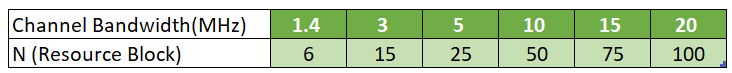
\includegraphics[width=1\linewidth]{graphics/bandwithandRB}
    \caption[Relatie tussen bandbreedte en resource blocks]{Relatie tussen bandbreedte en resource blocks \autocite{Kovadloff2021}}
    \label{fig:bandwithandrb}
\end{figure*}

Wanneer men wil bepalen in welke capaciteit een bepaald bericht kan getransporteerd worden over een netwerk is het belangrijk om de ruis aanwezig ook in te calculeren. Een maat staaf die daarvoor kan ingezet worden is Signal to Noise Ratio (SNR). Dit geeft een ratio weer van de signaal sterkte ten opzichte van de ruis aanwezig. Deze waarde word zoals de voorgaande weergegeven in dBm. Afgaande van hoe het ratio is opgesteld is ook duidelijk dat hoe dichter deze waarde nadert bij de nul, hoe slechter het netwerk er aan toe is en er een lagere kans is dat een bepaald object ook effectief kan verstuurd worden.  \autocite{Sheldon2021}

% Dit hoofdstuk bevat je literatuurstudie. De inhoud gaat verder op de inleiding, maar zal het onderwerp van de bachelorproef *diepgaand* uitspitten. De bedoeling is dat de lezer na lezing van dit hoofdstuk helemaal op de hoogte is van de huidige stand van zaken (state-of-the-art) in het onderzoeksdomein. Iemand die niet vertrouwd is met het onderwerp, weet nu voldoende om de rest van het verhaal te kunnen volgen, zonder dat die er nog andere informatie moet over opzoeken \autocite{Pollefliet2011}.

% Je verwijst bij elke bewering die je doet, vakterm die je introduceert, enz.\ naar je bronnen. In \LaTeX{} kan dat met het commando \texttt{$\backslash${textcite\{\}}} of \texttt{$\backslash${autocite\{\}}}. Als argument van het commando geef je de ``sleutel'' van een ``record'' in een bibliografische databank in het Bib\LaTeX{}-formaat (een tekstbestand). Als je expliciet naar de auteur verwijst in de zin (narratieve referentie), gebruik je \texttt{$\backslash${}textcite\{\}}. Soms is de auteursnaam niet expliciet een onderdeel van de zin, dan gebruik je \texttt{$\backslash${}autocite\{\}} (referentie tussen haakjes). Dit gebruik je bv.~bij een citaat, of om in het bijschrift van een overgenomen afbeelding, broncode, tabel, enz. te verwijzen naar de bron. In de volgende paragraaf een voorbeeld van elk.

% \textcite{Knuth1998} schreef een van de standaardwerken over sorteer- en zoekalgoritmen. Experten zijn het erover eens dat cloud computing een interessante opportuniteit vormen, zowel voor gebruikers als voor dienstverleners op vlak van informatietechnologie~\autocite{Creeger2009}.

% Let er ook op: het \texttt{cite}-commando voor de punt, dus binnen de zin. Je verwijst meteen naar een bron in de eerste zin die erop gebaseerd is, dus niet pas op het einde van een paragraaf.
